\documentclass{beamer}
\usepackage[utf8]{inputenc}
\usepackage{graphicx, epsfig}
\usepackage{amsmath,mathrsfs,amsfonts,amssymb}
\usepackage{floatflt}
\usepackage{epic,ecltree}
\usepackage{mathtext}
\usepackage{fancybox}
\usepackage{fancyhdr}
\usepackage{multirow}
\usepackage{enumerate}
\usepackage{epstopdf}
\usepackage{multicol}
\usepackage{algorithm}
\usepackage[noend]{algorithmic}
\usepackage{tikz}
\usepackage{blindtext}
\usetheme{default}%{Singapore}%{Warsaw}%{Warsaw}%{Darmstadt}
\usecolortheme{default}

\setbeamerfont{title}{size=\Huge}
\setbeamertemplate{footline}[page number]{}

\setbeamertemplate{section in toc}[sections numbered]


\makeatletter
\newcommand\HUGE{\@setfontsize\Huge{35}{40}}
\makeatother    

\setbeamerfont{title}{size=\HUGE}
\beamertemplatenavigationsymbolsempty

% latin bold lower
\newcommand{\ba}{\mathbf{a}} 
\newcommand{\bc}{\mathbf{c}} 
\newcommand{\be}{\mathbf{e}} 
\newcommand{\bh}{\mathbf{h}} 
\newcommand{\bp}{\mathbf{p}} 
\newcommand{\bt}{\mathbf{t}} 
\newcommand{\bs}{\mathbf{s}} 
\newcommand{\bu}{\mathbf{u}} 
\newcommand{\bv}{\mathbf{v}} 
\newcommand{\bw}{\mathbf{w}} 
\newcommand{\bx}{\mathbf{x}} 
\newcommand{\by}{\mathbf{y}} 
\newcommand{\bz}{\mathbf{z}} 

% latin bold upper
\newcommand{\bA}{\mathbf{A}} 
\newcommand{\bB}{\mathbf{B}} 
\newcommand{\bC}{\mathbf{C}} 
\newcommand{\bI}{\mathbf{I}} 
\newcommand{\bJ}{\mathbf{J}} 
\newcommand{\bL}{\mathbf{L}} 
\newcommand{\bM}{\mathbf{M}} 
\newcommand{\bP}{\mathbf{P}}
\newcommand{\bQ}{\mathbf{Q}} 
\newcommand{\bR}{\mathbf{R}} 
\newcommand{\bT}{\mathbf{T}} 
\newcommand{\bU}{\mathbf{U}} 
\newcommand{\bV}{\mathbf{V}} 
\newcommand{\bW}{\mathbf{W}} 
\newcommand{\bX}{\mathbf{X}} 
\newcommand{\bY}{\mathbf{Y}} 
\newcommand{\bZ}{\mathbf{Z}} 

% latin cal upper
\newcommand{\cF}{\mathcal{F}} 
\newcommand{\cG}{\mathcal{G}} 
\newcommand{\cI}{\mathcal{I}} 
\newcommand{\cL}{\mathcal{L}} 
\newcommand{\cM}{\mathcal{M}} 
\newcommand{\cN}{\mathcal{N}} 
\newcommand{\cP}{\mathcal{P}} 
\newcommand{\cS}{\mathcal{S}} 
\newcommand{\cT}{\mathcal{T}} 
\newcommand{\cW}{\mathcal{W}} 
\newcommand{\cX}{\mathcal{X}} 
\newcommand{\cZ}{\mathcal{Z}} 

% latin bb upper
\newcommand{\bbE}{\mathbb{E}} 
\newcommand{\bbI}{\mathbb{I}} 
\newcommand{\bbP}{\mathbb{P}} 
\newcommand{\bbR}{\mathbb{R}} 

% greek bold lower
\newcommand{\bepsilon}{\boldsymbol{\epsilon}} 
\newcommand{\btheta}{\boldsymbol{\theta}} 
\newcommand{\blambda}{\boldsymbol{\lambda}} 
\newcommand{\bpi}{\boldsymbol{\pi}} 
\newcommand{\bmu}{\boldsymbol{\mu}} 
\newcommand{\bsigma}{\boldsymbol{\sigma}} 
\newcommand{\bphi}{\boldsymbol{\phi}} 

% greek bold upper
\newcommand{\bSigma}{\boldsymbol{\Sigma}} 

\DeclareMathOperator*{\argmin}{arg\,min}
\DeclareMathOperator*{\argmax}{arg\,max}

\newcommand{\createdgmtitle}[1]{\title[\hbox to 56mm{Deep Generative Models  \hfill\insertframenumber\,/\,\inserttotalframenumber}]
	{\vspace{1cm} \\ \textbf{Deep Generative Models} \\ {\Huge Lecture #1}}
	\author{Roman Isachenko}
		\institute{
\includegraphics[width=0.7cm]{../utils/aimasterslogo} \LARGE{AI Masters}}
	\date{2024, Spring}
}

\usepackage{tikz}
\usetikzlibrary{arrows,shapes,positioning,shadows,trees}

\newcommand\myfootnote[1]{%
  \tikz[remember picture,overlay]
  \draw (current page.south west) +(1in + \oddsidemargin,0.5em)
  node[anchor=south west,inner sep=0pt]{\parbox{\textwidth}{%
      \rlap{\rule{10em}{0.4pt}}\raggedright\scriptsize \textit{#1}}};}

\newcommand\myfootnotewithlink[2]{%
  \tikz[remember picture,overlay]
  \draw (current page.south west) +(1in + \oddsidemargin,0.5em)
  node[anchor=south west,inner sep=0pt]{\parbox{\textwidth}{%
      \rlap{\rule{10em}{0.4pt}}\raggedright\scriptsize\href{#1}{\textit{#2}}}};}
      
\AtBeginSection[]
      {
      	\begin{frame}{Outline}
      		\tableofcontents[currentsection]
      	\end{frame}
      }
      \AtBeginSubsection[]{
      	\begin{frame}{Outline}
      		\tableofcontents[currentsection,currentsubsection]
      	\end{frame}
}
\createdgmtitle{7}
\usepackage{tikz}

\usetikzlibrary{arrows,shapes,positioning,shadows,trees}
%--------------------------------------------------------------------------------
\begin{document}
%--------------------------------------------------------------------------------
\begin{frame}[noframenumbering,plain]
%\thispagestyle{empty}
\titlepage
\end{frame}
%=======
\begin{frame}{Recap of previous lecture}
	\begin{figure}
		\centering
		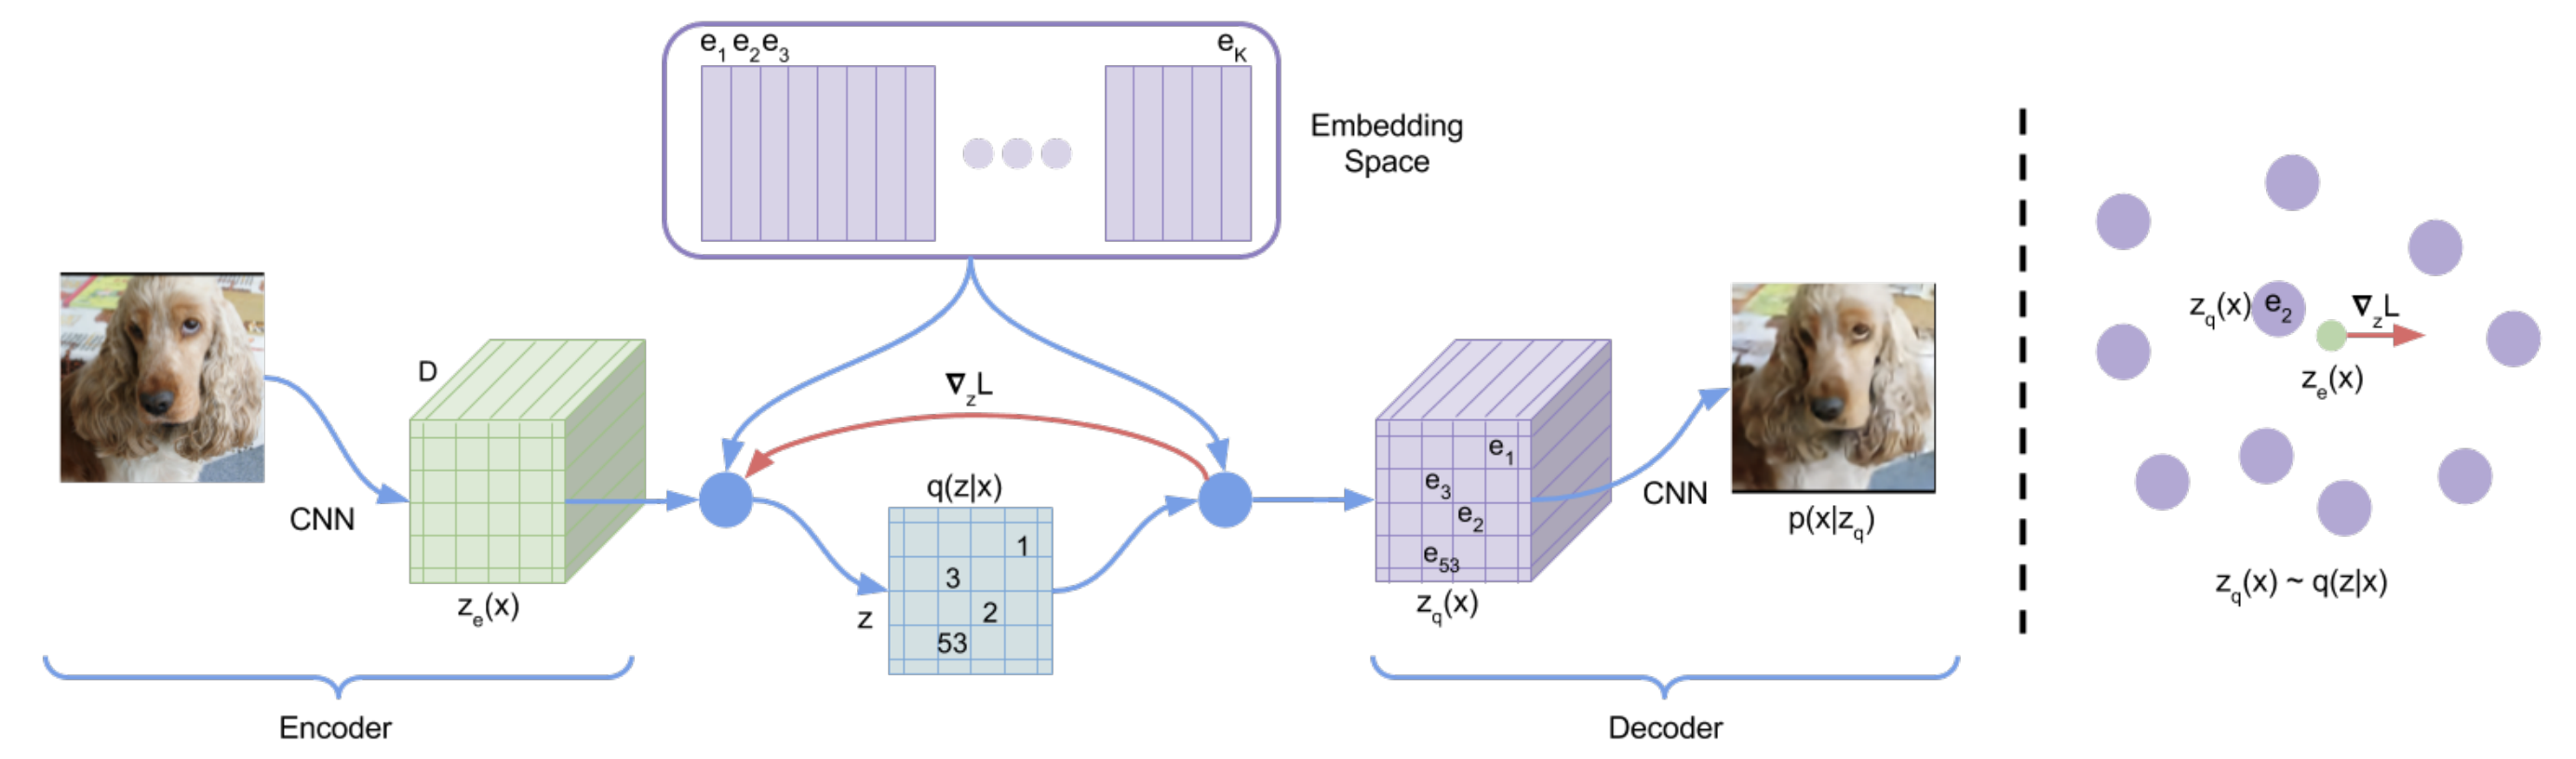
\includegraphics[width=0.85\linewidth]{figs/vqvae}
	\end{figure}
	\vspace{-0.3cm}
	\begin{block}{Deterministic variational posterior}
		\vspace{-0.8cm}
		\[
			q(c_{ij} = k^* | \bx, \bphi) = \begin{cases}
				1 , \quad \text{for } k^* = \argmin_k \| [\bz_e]_{ij} - \be_k \|; \\
				0, \quad \text{otherwise}.
			\end{cases}
		\]
		\vspace{-0.8cm}
	\end{block}
	\begin{block}{ELBO}
		\vspace{-0.6cm}
		\[
			\mathcal{L} (\bphi, \btheta)  = \mathbb{E}_{q(c | \bx, \bphi)} \log p(\bx | \be_{c} , \btheta) - \log K =  \log p(\bx | \bz_q, \btheta) - \log K.
		\]
		\vspace{-0.6cm}
	\end{block}
	\begin{block}{Straight-through gradient estimation}
		\vspace{-0.6cm}
		\[
			\frac{\partial \log p(\bx | \bz_q , \btheta)}{\partial \bphi} = \frac{\partial \log p(\bx | \bz_q, \btheta)}{\partial \bz_q} \cdot {\color{red}\frac{\partial \bz_q}{\partial \bphi}} \approx \frac{\partial \log p(\bx | \bz_q, \btheta)}{\partial \bz_q} \cdot \frac{\partial \bz_e}{\partial \bphi}
		\]
	\end{block}
	\myfootnotewithlink{https://arxiv.org/abs/1711.00937}{Oord A., Vinyals O., Kavukcuoglu K. Neural Discrete Representation Learning, 2017} 
\end{frame}
%=======
\begin{frame}{Recap of previous lecture}
	\vspace{-0.4cm}
	\begin{block}{Gumbel-max trick}
		Let $g_k \sim \text{Gumbel}(0, 1)$ for $k = 1, \dots, K$. Then
		\vspace{-0.3cm}
		\[
			c = \argmax_k [\log \pi_k + g_k]
		\]
		\vspace{-0.6cm} \\
		has a categorical distribution $c \sim \text{Categorical}(\bpi)$.
	\end{block}
	\vspace{-0.2cm}
	\begin{block}{Gumbel-softmax relaxation}
		{\color{violet}Con}{\color{teal}crete} distribution = {\color{violet}\textbf{con}tinuous} + {\color{teal}dis\textbf{crete}}
		\vspace{-0.2cm}
		\[
			\hat{c}_k = \frac{\exp \left(\frac{\log q(k | \bx, \bphi) + g_k}{\tau}\right)}{\sum_{j=1}^K \exp \left(\frac{\log q(j | \bx, \bphi) + g_j}{\tau}\right)}, \quad k = 1, \dots, K.
		\]
		\vspace{-0.7cm}
 	\end{block}
	\begin{block}{Reparametrization trick}
		\vspace{-0.4cm}
		\[
			\nabla_{\bphi} \mathbb{E}_{q(c | \bx, \bphi)} \log p(\bx | \be_{c} , \btheta) = \bbE_{\text{Gumbel}(0, 1)} \nabla_{\bphi} \log p(\bx | \bz , \btheta),
		\]
		where $\bz = \sum_{k=1}^K\hat{c}_k \be_k$ (all operations are differentiable now).
	\end{block}
 	\vspace{-0.2cm}
	\myfootnote{
	\href{https://arxiv.org/abs/1611.00712}{Maddison C. J., Mnih A., Teh Y. W. The Concrete distribution: A continuous relaxation of discrete random variables, 2016} \\
	\href{https://arxiv.org/abs/1611.01144}{Jang E., Gu S., Poole B. Categorical reparameterization with Gumbel-Softmax, 2016}
	}
\end{frame}
%=======
\begin{frame}{Recap of previous lecture}
	\begin{block}{Likelihood-free learning}
		\begin{itemize}
			\item Likelihood is not a perfect quality measure for generative model.
			\item Likelihood could be intractable.
		\end{itemize}
	\end{block}
	Imagine we have two sets of samples 
	\begin{itemize}
		\item $\cS_1 = \{\bx_i\}_{i=1}^{n_1} \sim \pi(\bx)$ -- real samples;
		\item $\cS_2 = \{\bx_i\}_{i=1}^{n_2} \sim p(\bx | \btheta)$ -- generated (or fake) samples.
	\end{itemize}
	Let define discriminative model (classifier):
	\[
		p(y = 1 | \bx) = P\bigl(\{\bx \sim \pi(\bx)\}\bigr); \quad p(y = 0 | \bx) = P\bigl(\{\bx \sim p(\bx | \btheta)\}\bigr)
	\]
	\vspace{-0.5cm}
	\begin{block}{Assumption}
		Generative distribution $p(\bx | \btheta)$ equals to the true distribution $\pi(\bx)$ if we can not distinguish them using discriminative model $p(y | \bx)$. \\
		It means that $p(y = 1 | \bx) = 0.5$ for each sample $\bx$.
	\end{block}
\end{frame}
%=======
\begin{frame}{Outline}
	\tableofcontents
\end{frame}
%=======
\section{Generative adversarial networks (GAN)}
%=======
\begin{frame}{Generative models zoo}
	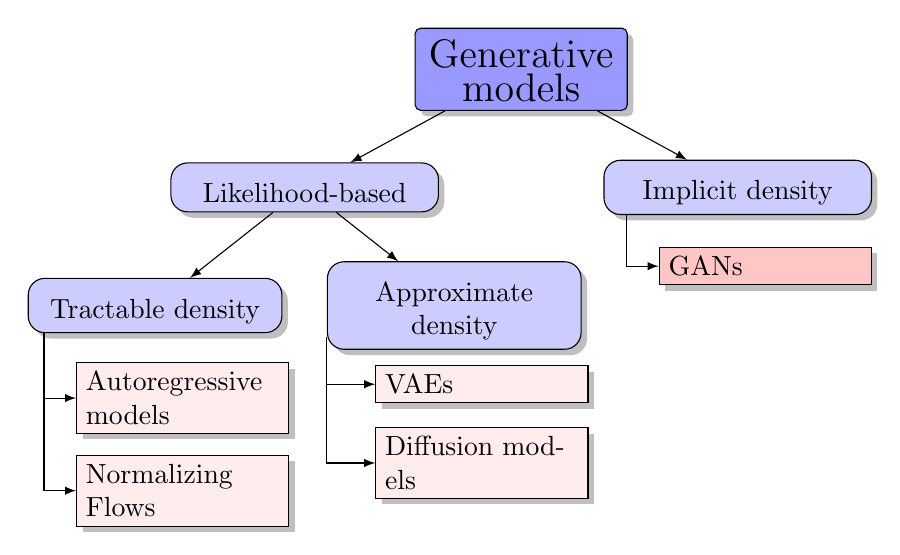
\begin{tikzpicture}[
	 	basic/.style  = {draw, text width=2cm, drop shadow, rectangle},
	 	root/.style   = {basic, rounded corners=2pt, thin, text height=1.1em, text width=7em, align=center, fill=blue!40},
	 	level 1/.style={sibling distance=55mm},
	 	level 2/.style = {basic, rounded corners=6pt, thin, align=center, fill=blue!20, text height=1.1em, text width=9em, sibling distance=38mm},
	 	level 3/.style = {basic, rounded corners=6pt, thin,align=center, fill=blue!20, text width=8.5em},
	 	level 4/.style = {basic, thin, align=left, fill=pink!30, text width=7em},
	 	level 5/.style = {basic, thin, align=left, fill=pink!90, text width=7em},
		edge from parent/.style={->,draw},
		>=latex]
		
		% root of the the initial tree, level 1
		\node[root] {\Large Generative models}
		% The first level, as children of the initial tree
		child {node[level 2] (c1) {Likelihood-based}
			child {node[level 3] (c11) {Tractable density}}
			child {node[level 3] (c12) {Approximate density}}
		}
		child {node[level 2] (c2) {Implicit density}};
		
		% The second level, relatively positioned nodes
		\begin{scope}[every node/.style={level 4}]
		\node [below of = c11, yshift=-5pt, xshift=10pt] (c111) {Autoregressive models};
		\node [below of = c111, yshift=-5pt] (c112) {Normalizing Flows};
		
		\node [below of = c12, xshift=10pt] (c121) {VAEs};
		\node [below of = c121] (c122) {Diffusion models};
		
		\end{scope}
		
		% The second level, relatively positioned nodes
		\begin{scope}[every node/.style={level 5}]
		\node [below of = c2, xshift=10pt] (c21) {GANs};
		\end{scope}
		
		
		% lines from each level 1 node to every one of its "children"
		\foreach \value in {1,2}
		\draw[->] (c11.194) |- (c11\value.west);
		
		\foreach \value in {1,2}
		\draw[->] (c12.194) |- (c12\value.west);
		
		\draw[->] (c2.194) |- (c21.west);
		
	\end{tikzpicture}
\end{frame}
%=======
\begin{frame}{GAN optimality}
	\begin{block}{Theorem}
		The minimax game 
		\vspace{-0.3cm}
		\[
			\min_{G} \max_D \Bigl[ \underbrace{\bbE_{\pi(\bx)} \log D(\bx) + \bbE_{p(\bz)} \log (1 - D(G(\bz)))}_{V(G, D)} \Bigr]
		\]
		\vspace{-0.5cm} \\
		has the global optimum $\pi(\bx) = p(\bx | \btheta)$, in this case $D^*(\bx) = 0.5$.
	\end{block}
	\begin{block}{Proof (fixed $G$)}
		\vspace{-0.5cm}
		\begin{align*}
			V(G, D) &= \bbE_{\pi(\bx)} \log D(\bx) + \bbE_{p(\bx | \btheta)} \log (1 - D(\bx)) \\
			&= \int \underbrace{\left[ \pi(\bx) \log D(\bx) + p(\bx | \btheta)\log (1 - D(\bx) \right]}_{y(D)} d \bx
		\end{align*}
		\vspace{-0.2cm}
		\[
			\frac{d y(D)}{d D} = \frac{\pi(\bx)}{D(\bx)} - \frac{p(\bx | \btheta)}{1 - D(\bx)} = 0 \quad \Rightarrow \quad D^*(\bx) = \frac{\pi(\bx)}{\pi(\bx) + p(\bx | \btheta)}
		\]
	\end{block}
	\myfootnotewithlink{https://arxiv.org/abs/1406.2661}{Goodfellow I. J. et al. Generative Adversarial Networks, 2014}
\end{frame}
%=======
\begin{frame}{GAN optimality}
	\begin{block}{Proof continued (fixed $D = D^*$)}
		\vspace{-0.5cm}
		\begin{multline*}
			V(G, D^*) = \bbE_{\pi(\bx)} \log \left( \frac{\pi(\bx)}{\pi(\bx) + p(\bx | \btheta)} \right) + \bbE_{p(\bx | \btheta)} \log \left( \frac{p(\bx | \btheta)}{\pi(\bx) + p(\bx | \btheta)}\right)  \\
		 = KL \left(\pi(\bx) || \frac{\pi(\bx) + p(\bx | \btheta)}{2}\right) + KL \left(p(\bx | \btheta) || \frac{\pi(\bx) + p(\bx | \btheta)}{2}\right) - 2\log 2 \\
		 = 2JSD(\pi(\bx) || p(\bx | \btheta)) - 2\log 2.
		\end{multline*}
	\end{block}
	\vspace{-0.3cm}
	\begin{block}{Jensen-Shannon divergence (symmetric KL divergence)}
		\vspace{-0.2cm}
		\footnotesize
		\[
			JSD(\pi(\bx) || p(\bx | \btheta)) = \frac{1}{2} \left[KL \left(\pi(\bx) || \frac{\pi(\bx) + p(\bx | \btheta)}{2}\right) + KL \left(p(\bx | \btheta) || \frac{\pi(\bx) + p(\bx | \btheta)}{2}\right) \right]
		\]
	\end{block}
	Could be used as a distance measure!
	\[
		V(G^*, D^*) = -2\log 2, \quad \pi(\bx) = p(\bx | \btheta), \quad  D^*(\bx) = 0.5.
	\]
	
	 \myfootnotewithlink{https://arxiv.org/abs/1406.2661}{Goodfellow I. J. et al. Generative Adversarial Networks, 2014}
\end{frame}
%=======
\begin{frame}{GAN optimality}
	\begin{block}{Theorem}
		The minimax game 
		\vspace{-0.3cm}
		\[
		\min_{G} \max_D \Bigl[ \underbrace{\bbE_{\pi(\bx)} \log D(\bx) + \bbE_{p(\bz)} \log (1 - D(G(\bz)))}_{V(G, D)} \Bigr]
		\]
		\vspace{-0.5cm} \\
		has the global optimum $\pi(\bx) = p(\bx | \btheta)$, in this case $D^*(\bx) = 0.5$.
	\end{block}
	\vspace{-0.2cm}
	\begin{block}{Expectations}
		If the generator could be \textbf{any} function and the discriminator is \textbf{optimal} at every step, then the generator is \textbf{guaranteed to converge} to the data distribution.
	\end{block}
	\begin{block}{Reality}
		\begin{itemize}
			\item Generator updates are made in parameter space, discriminator is not optimal at every step.
			\item Generator and discriminator loss keeps oscillating during GAN training.
		\end{itemize}
	\end{block}
	 \myfootnotewithlink{https://arxiv.org/abs/1406.2661}{Goodfellow I. J. et al. Generative Adversarial Networks, 2014}
\end{frame}
%=======
\begin{frame}{GAN training}
	Let further assume that generator and discriminator are parametric models: $D_{\bphi}(\bx)$ and $G_{\btheta}(\bz)$.
	\begin{block}{Objective}
		\vspace{-0.7cm}
		\[
		\min_{\btheta} \max_{\bphi} \left[ \bbE_{\pi(\bx)} \log D_{\bphi}(\bx) + \bbE_{p(\bz)} \log (1 - D_{\bphi}(G_{\btheta}(\bz))) \right]
		\]
		\vspace{-0.7cm}
	\end{block}
	\begin{figure}
		\centering
		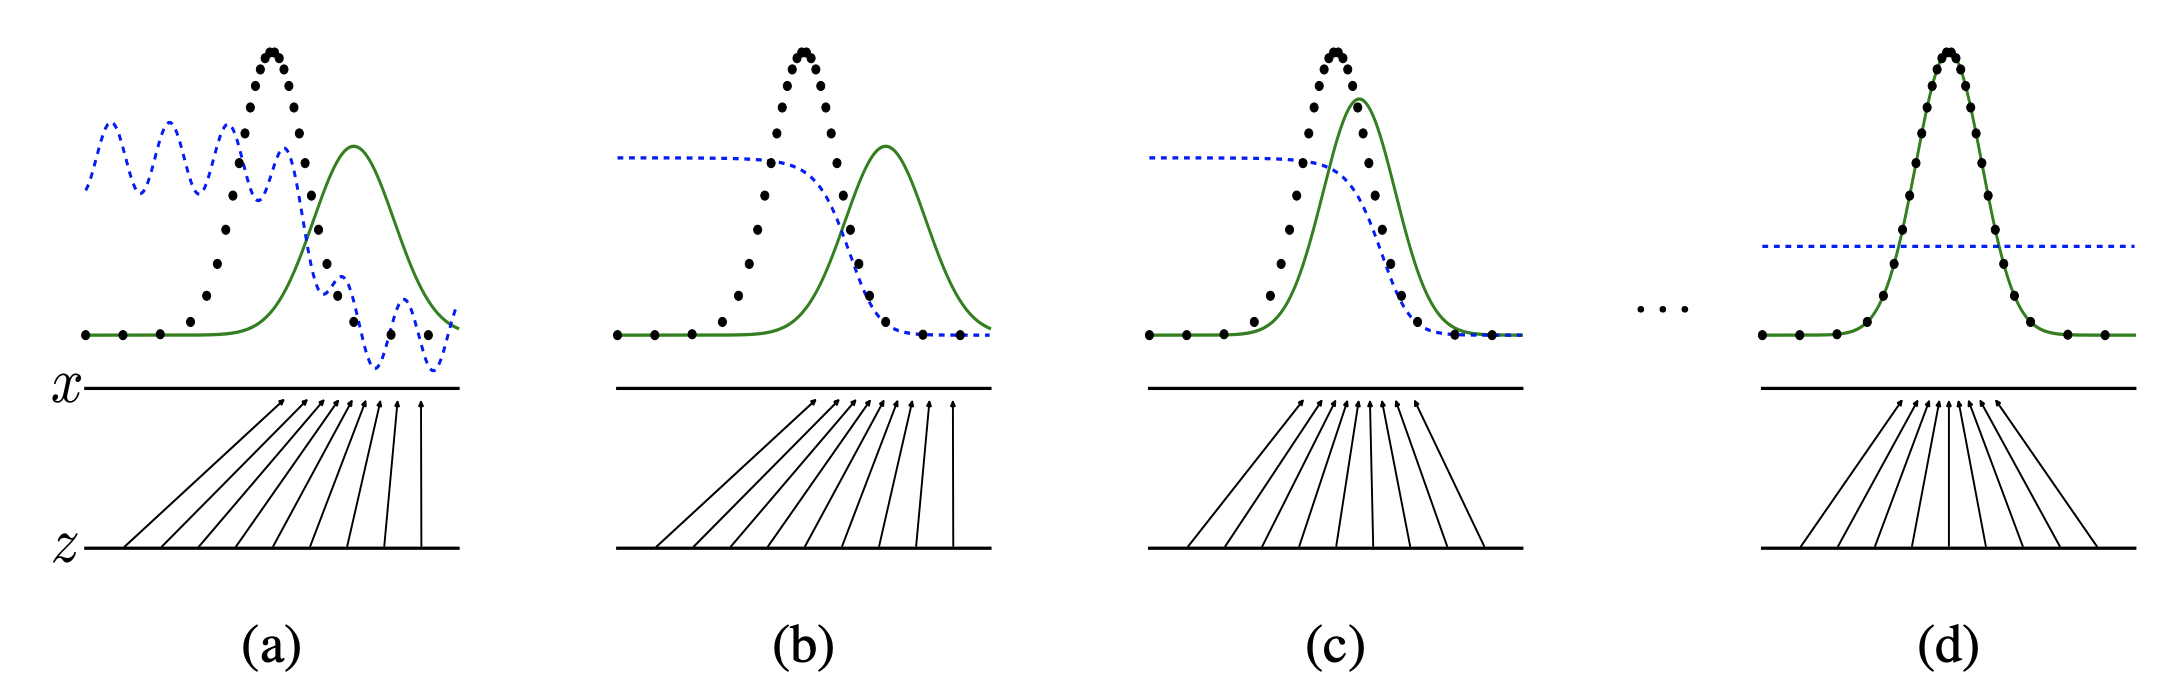
\includegraphics[width=1.0\linewidth]{figs/gan_1}
	\end{figure}

	\begin{itemize}
		\item $\bz \sim p(\bz)$ is a latent variable.
		\item $p(\bx | \bz, \btheta) = \delta(\bx - G_{\btheta}(\bz))$ is deterministic decoder ({\color{gray} like NF}).
		\item We do not have encoder at all.
	\end{itemize}

	 \myfootnotewithlink{https://arxiv.org/abs/1406.2661}{Goodfellow I. J. et al. Generative Adversarial Networks, 2014}
\end{frame}
%=======
\begin{frame}{Mode collapse}
	The phenomena where the generator of a GAN collapses to one or few distribution modes.
	\vspace{-0.15cm}
	\begin{figure}
		\centering
		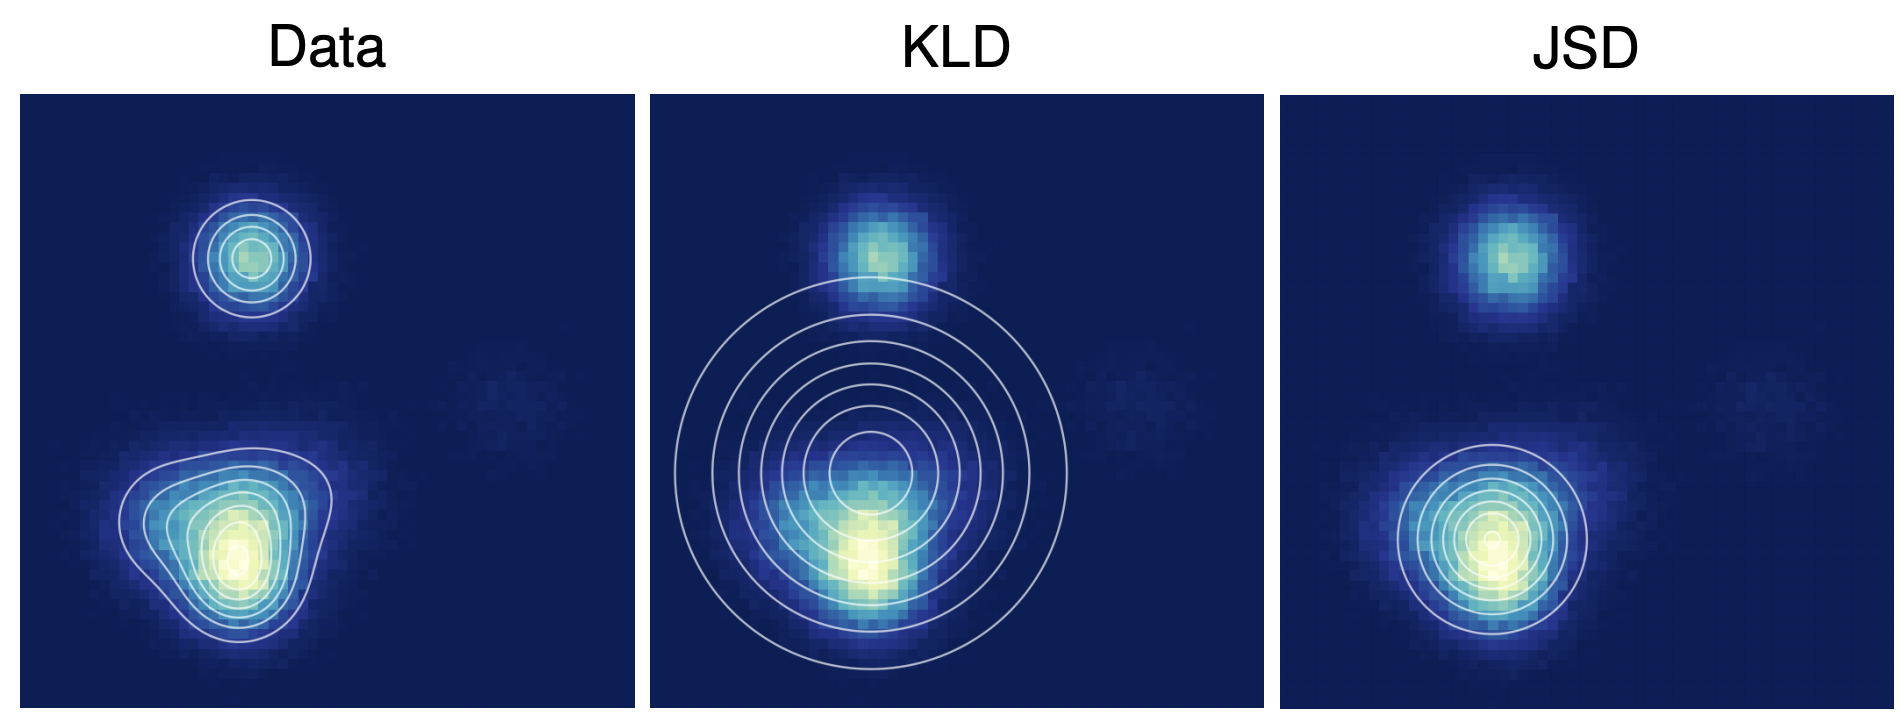
\includegraphics[width=0.75\linewidth]{figs/mode_collapse_1}
	\end{figure}
	\vspace{-0.3cm}
	\begin{figure}
		\centering
		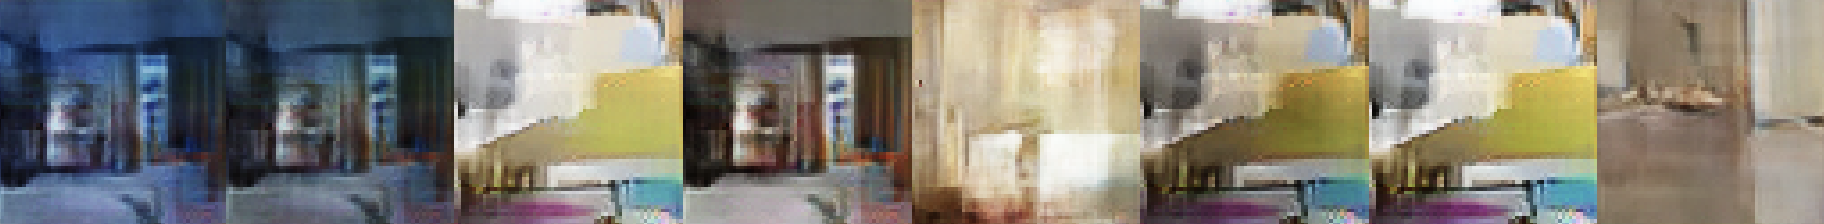
\includegraphics[width=1.0\linewidth]{figs/mode_collapse_4}
	\end{figure}
	Alternate architectures, adding regularization terms, injecting small noise
	perturbations and other millions bags and tricks are used to avoid the mode collapse.
	
	\myfootnote{\href{https://arxiv.org/abs/1406.2661}{Goodfellow I. J. et al. Generative Adversarial Networks, 2014} \\
		\href{https://arxiv.org/abs/1611.02163}{Metz L. et al. Unrolled Generative Adversarial Networks, 2016}}
\end{frame}
%=======
\begin{frame}{Jensen-Shannon vs Kullback-Leibler }
	\begin{itemize}
		\item $\pi(\bx)$ is a fixed mixture of 2 gaussians.
		\item $p(\bx | \mu, \sigma) - \cN(\mu, \sigma^2)$.
	\end{itemize}
	\begin{block}{Mode covering vs mode seeking}
		\vspace{-0.7cm}
		\[
		KL(\pi || p) = \int \pi(\bx) \log \frac{\pi(\bx)}{p(\bx)}d\bx, \quad KL(p || \pi) = \int p(\bx) \log \frac{p(\bx)}{\pi(\bx)}d\bx
		\]
		\[
		JSD(\pi || p) = \frac{1}{2} \left[KL \left(\pi(\bx) || \frac{\pi(\bx) + p(\bx)}{2}\right) + KL \left(p(\bx) || \frac{\pi(\bx) + p(\bx)}{2}\right) \right]
		\]
		\vspace{-0.7cm}
		
		\begin{minipage}[t]{0.33\columnwidth}
			\begin{figure}
				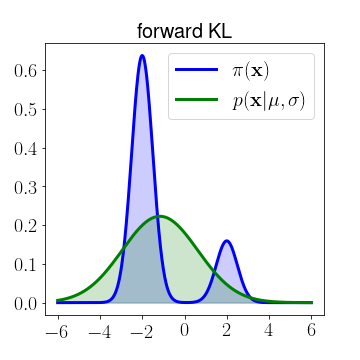
\includegraphics[width=\linewidth]{figs/forward_KL}
			\end{figure}
		\end{minipage}%
		\begin{minipage}[t]{0.33\columnwidth}
			\begin{figure}
				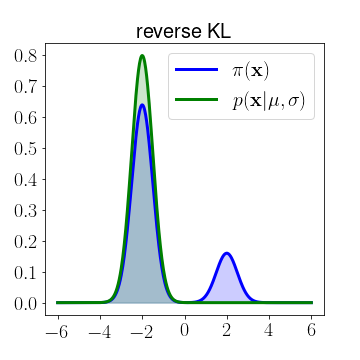
\includegraphics[width=\linewidth]{figs/reverse_KL}
			\end{figure}
		\end{minipage}%
		\begin{minipage}[t]{0.33\columnwidth}
			\begin{figure}
				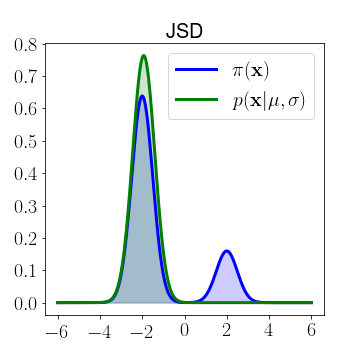
\includegraphics[width=\linewidth]{figs/JSD}
			\end{figure}
		\end{minipage}
		\vspace{-0.3cm}
	\end{block}
\end{frame}
%=======
\section{Wasserstein distance}
%=======
\begin{frame}{Informal theoretical results}
	\vspace{-0.3cm}
	\begin{itemize}
		\footnotesize
		\item Since $\bz$ usually has lower dimensionality compared to $\bx$, manifold $G_{\btheta}(\bz)$ has a measure 0 in $\bx$ space. Hence, support of $p(\bx | \btheta)$ lies on low-dimensional manifold.
		\item Distribution of real images $\pi(\bx)$ is also concentrated on a low dimensional manifold.
		\begin{figure}
			\centering
			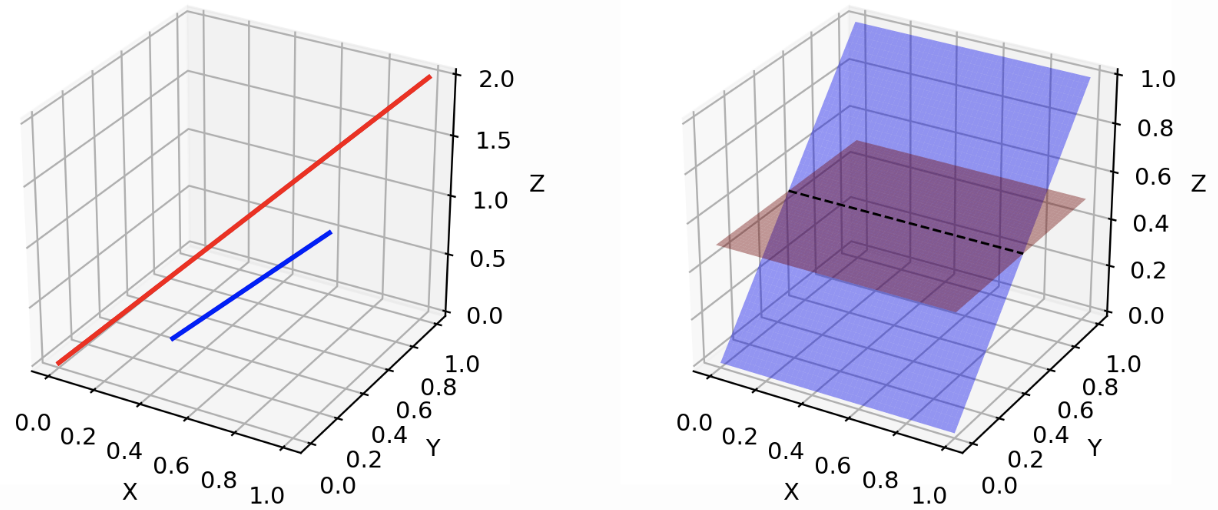
\includegraphics[width=0.5\linewidth]{figs/low_dim_manifold}
		\end{figure}
		\item If $\pi(\bx)$ and $p(\bx | \btheta)$ have disjoint supports, then there is a smooth optimal discriminator. We are not able to learn anything by backproping through it.
		\item For such low-dimensional disjoint manifolds
		\vspace{-0.2cm}
		\[
			KL(\pi || p) = KL(p || \pi) = \infty, \quad JSD(\pi || p) = \log 2
		\]
		\vspace{-0.7cm}
		\item Adding continuous noise to the inputs of the discriminator smoothes the distributions of the probability mass.
	\end{itemize}
	\myfootnote{\href{https://arxiv.org/abs/1904.08994}{Weng L. From GAN to WGAN, 2019} \\ 
	\href{https://arxiv.org/abs/1701.04862}{Arjovsky M., Bottou L. Towards Principled Methods for Training Generative Adversarial Networks, 2017}}
\end{frame}
%=======
\begin{frame}{Wasserstein distance (discrete)}
	A.k.a. \textbf{Earth Mover's distance}.
	The minimum cost of moving and transforming a pile of dirt in the shape of one probability distribution to the shape of the other distribution.
	\begin{figure}
		\centering
		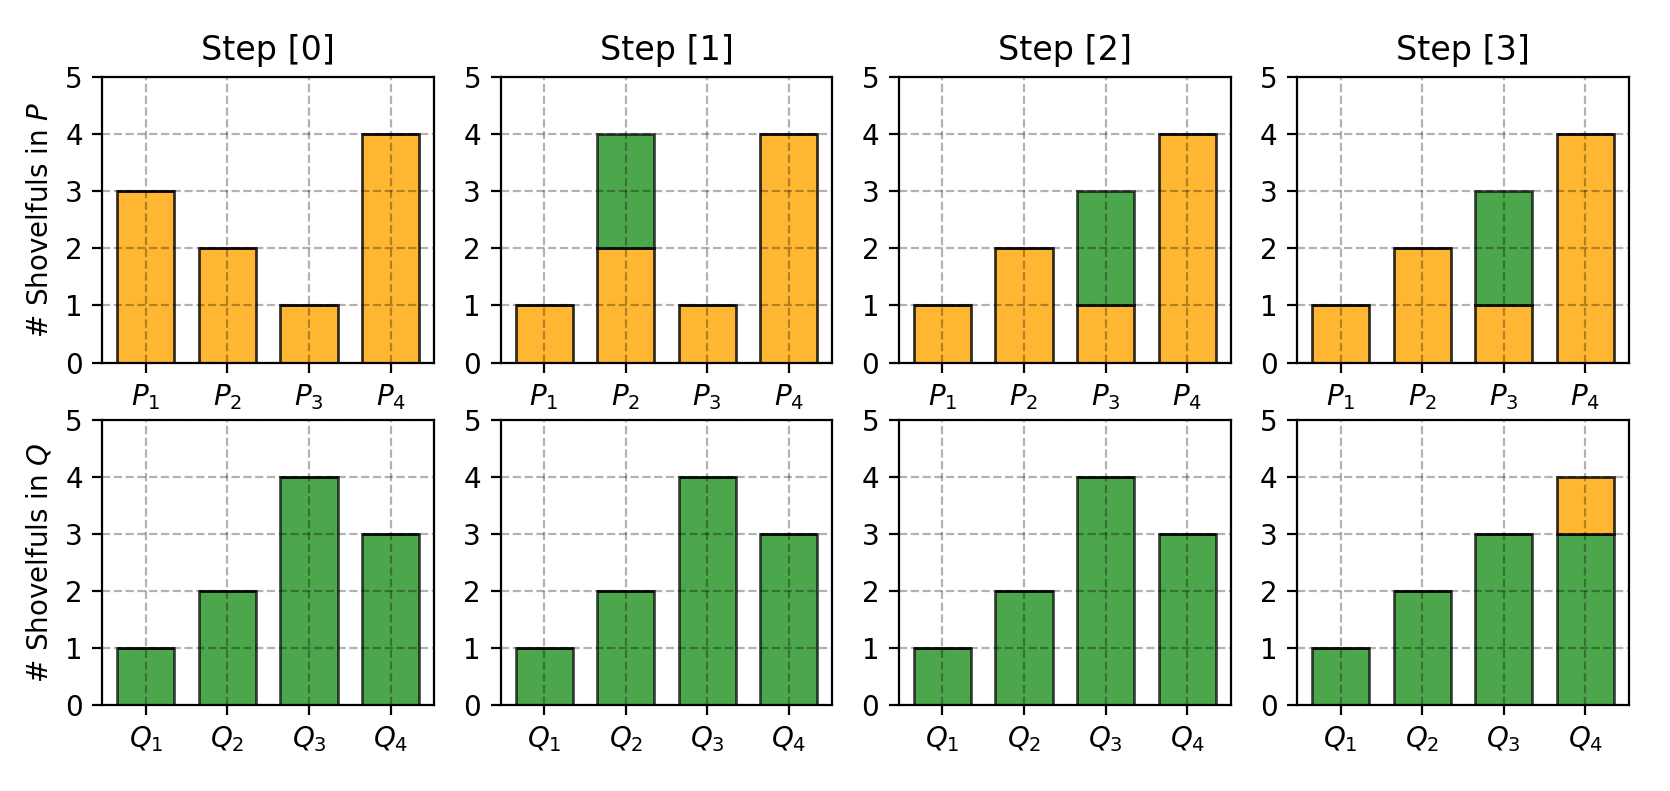
\includegraphics[width=.9\linewidth]{figs/EM_distance_discrete}
	\end{figure}
	\[
		W(P, Q) = 2 \text{(step 1)} + 2 \text{(step 2)} + 1 \text{(step 3)}  = 5
	\]
	\myfootnotewithlink{https://arxiv.org/abs/1904.08994}{Weng L. From GAN to WGAN, 2019} 
	
\end{frame}
%=======
\begin{frame}{Wasserstein distance (continuous)}
	\[
		W(\pi, p) = \inf_{\gamma \in \Gamma(\pi, p)} \bbE_{(\bx, \by) \sim \gamma} \| \bx - \by \| =  \inf_{{\color{olive}\gamma}\in {\color{teal}\Gamma(\pi, p)}} \int {\color{violet} \| \bx - \by \|} {\color{olive}\gamma (\bx, \by)} d \bx d \by
	\]
	\begin{itemize}
		\item ${\color{olive}\gamma (\bx, \by)}$ -- transportation plan (the amount of "dirt" that should be transported from point $\bx$ to point $\by$)
		\[
			 \int \gamma(\bx, \by) d \bx = p(\by); \quad \int \gamma(\bx, \by) d \by = \pi(\bx).
		\]
		\item ${\color{teal}\Gamma(\pi, p)}$ -- the set of all joint distributions $\gamma (\bx, \by)$ with marginals $\pi$ and $p$.
		\item ${\color{olive}\gamma(\bx, \by)}$ -- the amount, ${\color{violet} \| \bx - \by \|}$-- the distance.
	\end{itemize}
	{\color{gray}For better understanding of transportation plan function $\gamma$, try to write down the plan for previous discrete case.}
	\myfootnotewithlink{https://arxiv.org/abs/1701.07875}{Arjovsky M., Chintala S., Bottou L. Wasserstein GAN, 2017}
\end{frame}
%=======
\begin{frame}{Wasserstein distance vs KL vs JSD}
	
	\begin{minipage}[t]{0.48\columnwidth}
		\vspace{0.1cm}
		Consider 2d distributions
		\[
			\pi(x, y) = (0, U[0,1])
		\]	
		\[
			p(x, y | \theta) = (\theta, U[0, 1])
		\]
	\end{minipage}%
	\begin{minipage}[t]{0.52\columnwidth}
		\begin{figure}
			\centering
			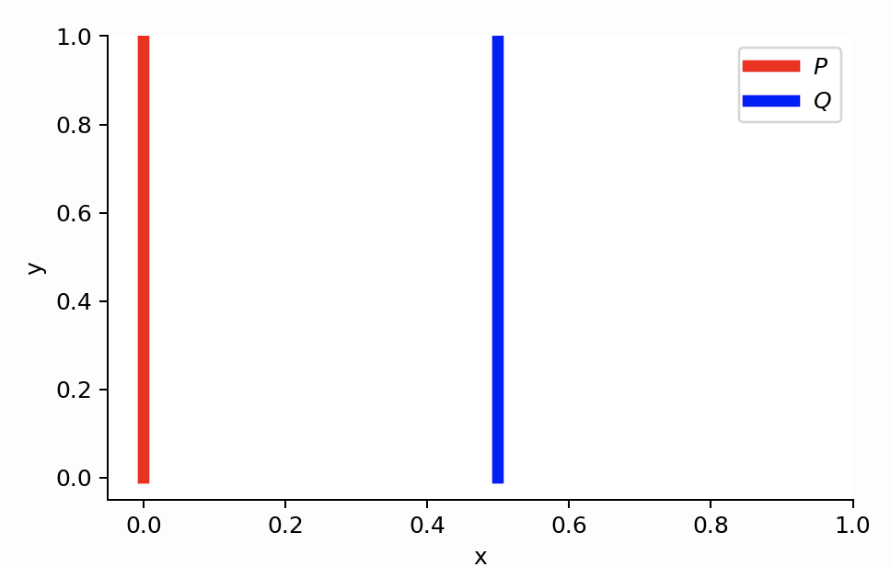
\includegraphics[width=0.8\linewidth]{figs/w_kl_jsd}
		\end{figure}
	\end{minipage}
	\begin{itemize}
		\footnotesize
		\item $\theta = 0$.
		Distributions are the same 
		\[
			KL(\pi || p) = KL(p || \pi) = JSD(p || \pi) = W(\pi, p) = 0
		\]
		\item $\theta \neq 0$
		\[
			KL(\pi || p) = \int_{U[0, 1]} 1 \log \frac{1}{0} d y = \infty = KL(p || \pi)
		\]
		\[
			JSD(\pi || p) = \frac{1}{2}\left( \int_{U[0, 1]}1 \log \frac{1}{1/2} dy + \int_{U[0, 1]}1 \log \frac{1}{1/2} dy \right) = \log 2
		\]
		\[
			W(\pi, p) = |\theta|
		\]
	\end{itemize}
	
	\myfootnote{\href{https://arxiv.org/abs/1904.08994}{Weng L. From GAN to WGAN, 2019} \\ 
	\href{https://arxiv.org/abs/1701.07875}{Arjovsky M., Chintala S., Bottou L. Wasserstein GAN, 2017}}
\end{frame}
%=======
\begin{frame}{Wasserstein distance vs KL vs JSD}
	\begin{block}{Theorem 1}
		Let $G_{\btheta}(\bz)$ be (almost) any feedforward neural network, and $p(\bz)$ a prior over $\bz$ such that $\bbE_{p(\bz)} \|\bz\| < \infty$. Then therefore $W(\pi, p)$ is continuous everywhere and differentiable almost everywhere.
	\end{block}
	\begin{block}{Theorem 2}
		Let $\pi$ be a distribution on a compact space $\cX$ and $\{p_t\}_{t=1}^\infty$ be a sequence of distributions on $\cX$. 
		\begin{align}
			KL(\pi || p_t) &\rightarrow 0 \, (\text{or }KL (p_t || \pi) \rightarrow 0) \\
			JSD(\pi || p_t) &\rightarrow 0 \\
			W(\pi || p_t) &\rightarrow 0
		\end{align}
		
		Then, considering limits as $t \rightarrow \infty$, (1) implies (2), (2) implies (3).
	\end{block}
	\myfootnotewithlink{https://arxiv.org/abs/1701.07875}{Arjovsky M., Chintala S., Bottou L. Wasserstein GAN, 2017}
\end{frame}
%=======
\begin{frame}{Wasserstein GAN}
	\begin{block}{Wasserstein distance}
		\vspace{-0.5cm}
		\[
			W(\pi || p) = \inf_{\gamma \in \Gamma(\pi, p)} \bbE_{(\bx, \by) \sim \gamma} \| \bx - \by \| =  \inf_{\gamma \in \Gamma(\pi, p)} \int \| \bx - \by \| \gamma (\bx, \by) d \bx d \by
		\]
		\vspace{-0.3cm}
	\end{block}
	The infimum across all possible joint distributions in $\Gamma(\pi, p)$ is intractable.
	\begin{block}{Theorem (Kantorovich-Rubinstein duality)}
		\vspace{-0.3cm}
		\[
			W(\pi || p) = \frac{1}{K} \max_{\| f \|_L \leq K} \left[ \bbE_{\pi(\bx)} f(\bx)  - \bbE_{p(\bx)} f(\bx)\right],
		\]
		where $\| f \|_L \leq K$ are $K-$Lipschitz continuous functions ($f: \cX \rightarrow \bbR$)
		\vspace{-0.2cm}
		\[
			|f(\bx_1) - f(\bx_2)| \leq K \| \bx_1 - \bx_2 \|, \quad \text{for all } \bx_1, \bx_2 \in \cX.
		\]
		\vspace{-0.5cm}
	\end{block}
	Now we need only samples to get Monte Carlo estimate for $W(\pi || p)$.

	\myfootnotewithlink{https://arxiv.org/abs/1701.07875}{Arjovsky M., Chintala S., Bottou L. Wasserstein GAN, 2017}
\end{frame}
%=======
\section{Lipschitzness of Wasserstein GAN critic}
%=======
\subsection{Wasserstein GAN}
%=======
\begin{frame}{Wasserstein GAN}
	\begin{block}{Theorem (Kantorovich-Rubinstein duality)}
		\[
		W(\pi || p) = \frac{1}{K} \max_{\| f \|_L \leq K} \left[ \bbE_{\pi(\bx)} f(\bx)  - \bbE_{p(\bx)} f(\bx)\right],
		\]
	\end{block}
	\begin{itemize}
		\item Now we have to ensure that $f$ is $K$-Lipschitz continuous.
		\item Let $f_{\bphi}(\bx)$ be a feedforward neural network parametrized by~$\bphi$.
		\item If parameters $\bphi$ lie in a compact set $\boldsymbol{\Phi}$ then $f_{\bphi}(\bx)$ will be $K$-Lipschitz continuous function. 
		\item Let the parameters be clamped to a fixed box $\boldsymbol{\Phi} \in [-c, c]^d$ (e.x. $c = 0.01$) after each gradient update.
	\end{itemize}
	\begin{multline*}
		K \cdot W(\pi || p) = \max_{\| f \|_L \leq K} \left[ \bbE_{\pi(\bx)} f(\bx)  - \bbE_{p(\bx)} f(\bx)\right] \geq \\  \geq \max_{\bphi \in \boldsymbol{\Phi}} \left[ \bbE_{\pi(\bx)} f_{\bphi}(\bx)  - \bbE_{p(\bx)} f_{\bphi}(\bx)\right]
	\end{multline*}
	
	\myfootnotewithlink{https://arxiv.org/abs/1701.07875}{Arjovsky M., Chintala S., Bottou L. Wasserstein GAN, 2017}
\end{frame}
%=======
\begin{frame}{Wasserstein GAN}
	\begin{block}{Standard GAN objective}
		\vspace{-0.2cm}
		\[
		\min_{\btheta} \max_{\bphi} \bbE_{\pi(\bx)} \log D_{\bphi}(\bx) + \bbE_{p(\bz)} \log (1 - D_{\bphi}(G_{\btheta}(\bz)))
		\]
		\vspace{-0.2cm}
	\end{block}
	\begin{block}{WGAN objective}
		\vspace{-0.3cm}
		\[
		\min_{\btheta} W(\pi || p) \approx \min_{\btheta} \max_{\bphi \in \boldsymbol{\Phi}} \left[ \bbE_{\pi(\bx)} f_{\bphi}(\bx)  - \bbE_{p(\bz)} f_{\bphi}(G_{\btheta}(\bz))\right].
		\]
		\vspace{-0.3cm}
	\end{block}
	\begin{itemize}
		\item Discriminator $D$ is similar to the function $f$, but not the same (it is not a classifier anymore). In the WGAN model, function~$f$ is usually called $\textbf{critic}$.
		\item \textit{"Weight clipping is a clearly terrible way to enforce a Lipschitz constraint"}. If the clipping parameter $c$ is too large, it is hard to train the critic till optimality. If the clipping parameter $c$ is too small, it could lead to vanishing gradients.
	\end{itemize}
	
	\myfootnotewithlink{https://arxiv.org/abs/1701.07875}{Arjovsky M., Chintala S., Bottou L. Wasserstein GAN, 2017}
\end{frame}
%=======
\begin{frame}{Wasserstein GAN}
	\begin{minipage}[t]{0.6\columnwidth}
		\begin{itemize}
			\item WGAN has non-zero gradients for disjoint supports.
			\item $JSD(\pi || p)$ correlates poorly with the sample quality. Stays constast nearly maximum value $\log 2 \approx 0.69$.
			\item $W(\pi || p)$ is highly correlated with the sample quality. 
		\end{itemize}
	\end{minipage}%
	\begin{minipage}[t]{0.4\columnwidth}
		\begin{figure}
			\centering
			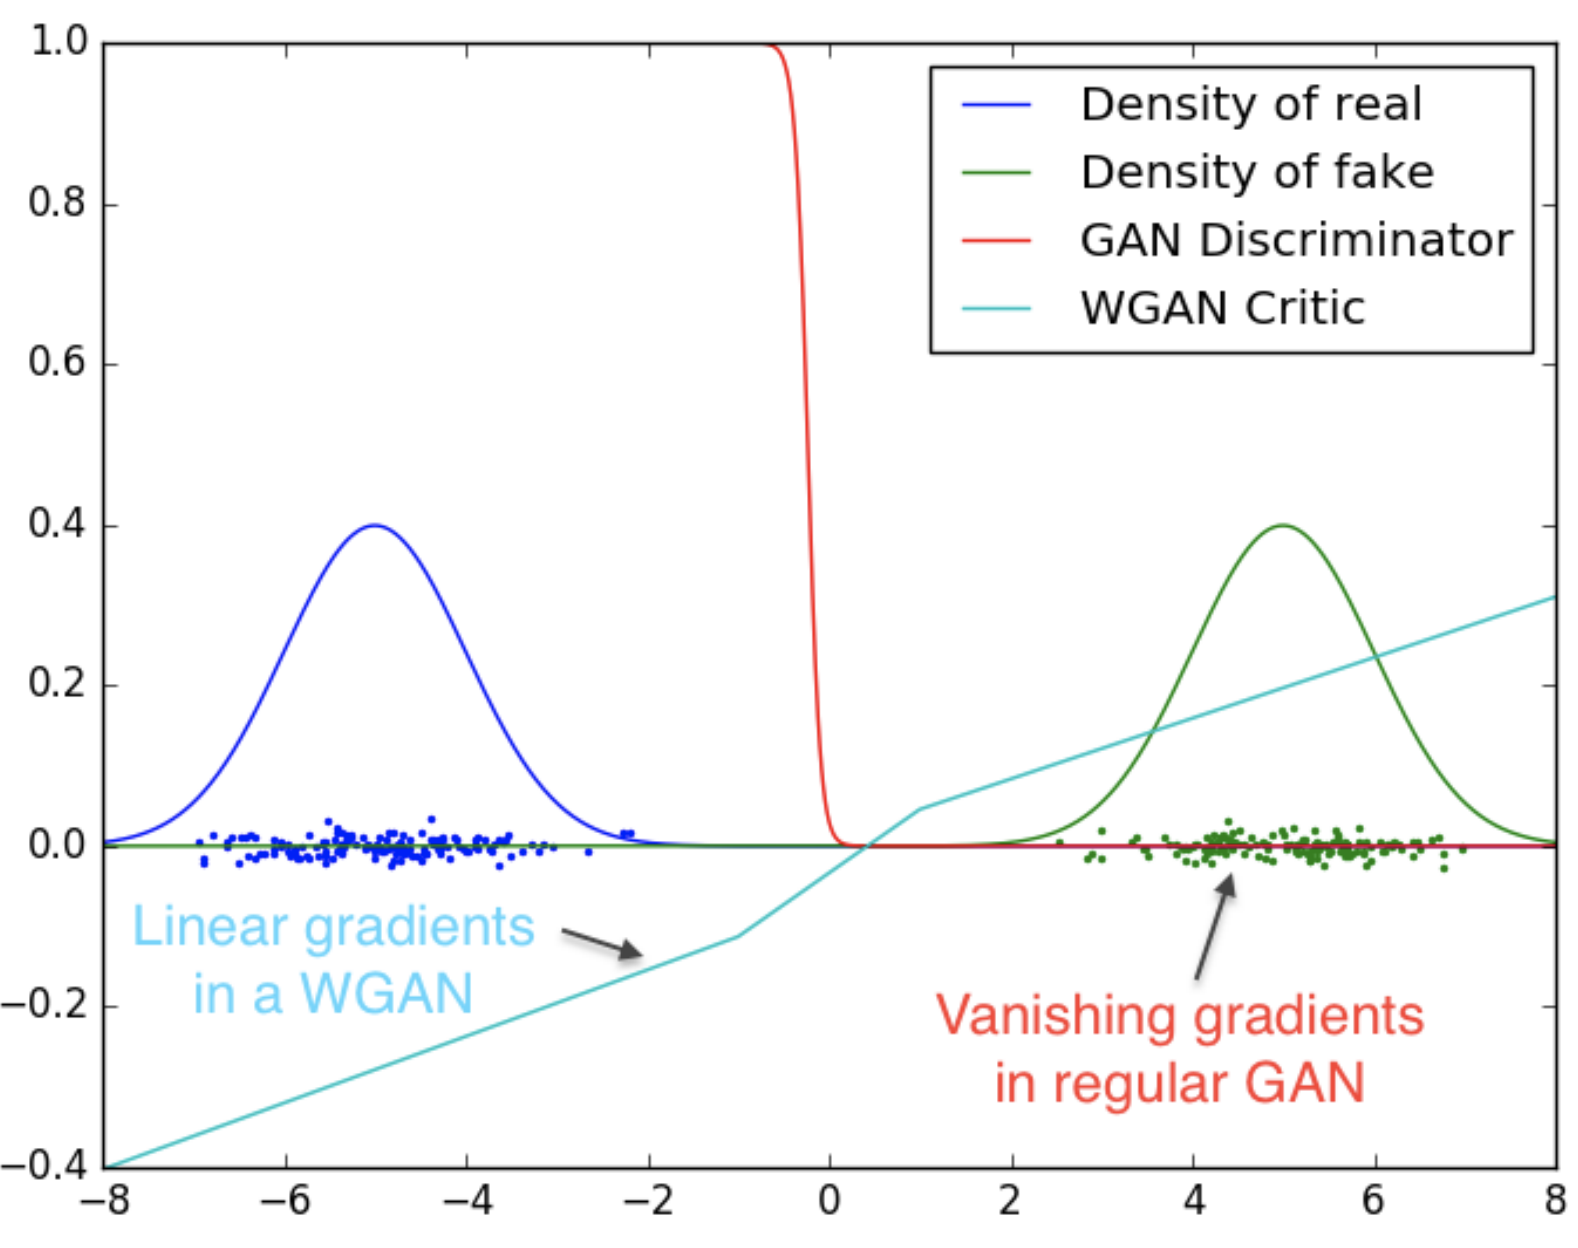
\includegraphics[width=\linewidth]{figs/wgan_toy}
		\end{figure}
	\end{minipage}
	\begin{minipage}[t]{0.5\columnwidth}
		\begin{figure}
			\centering
			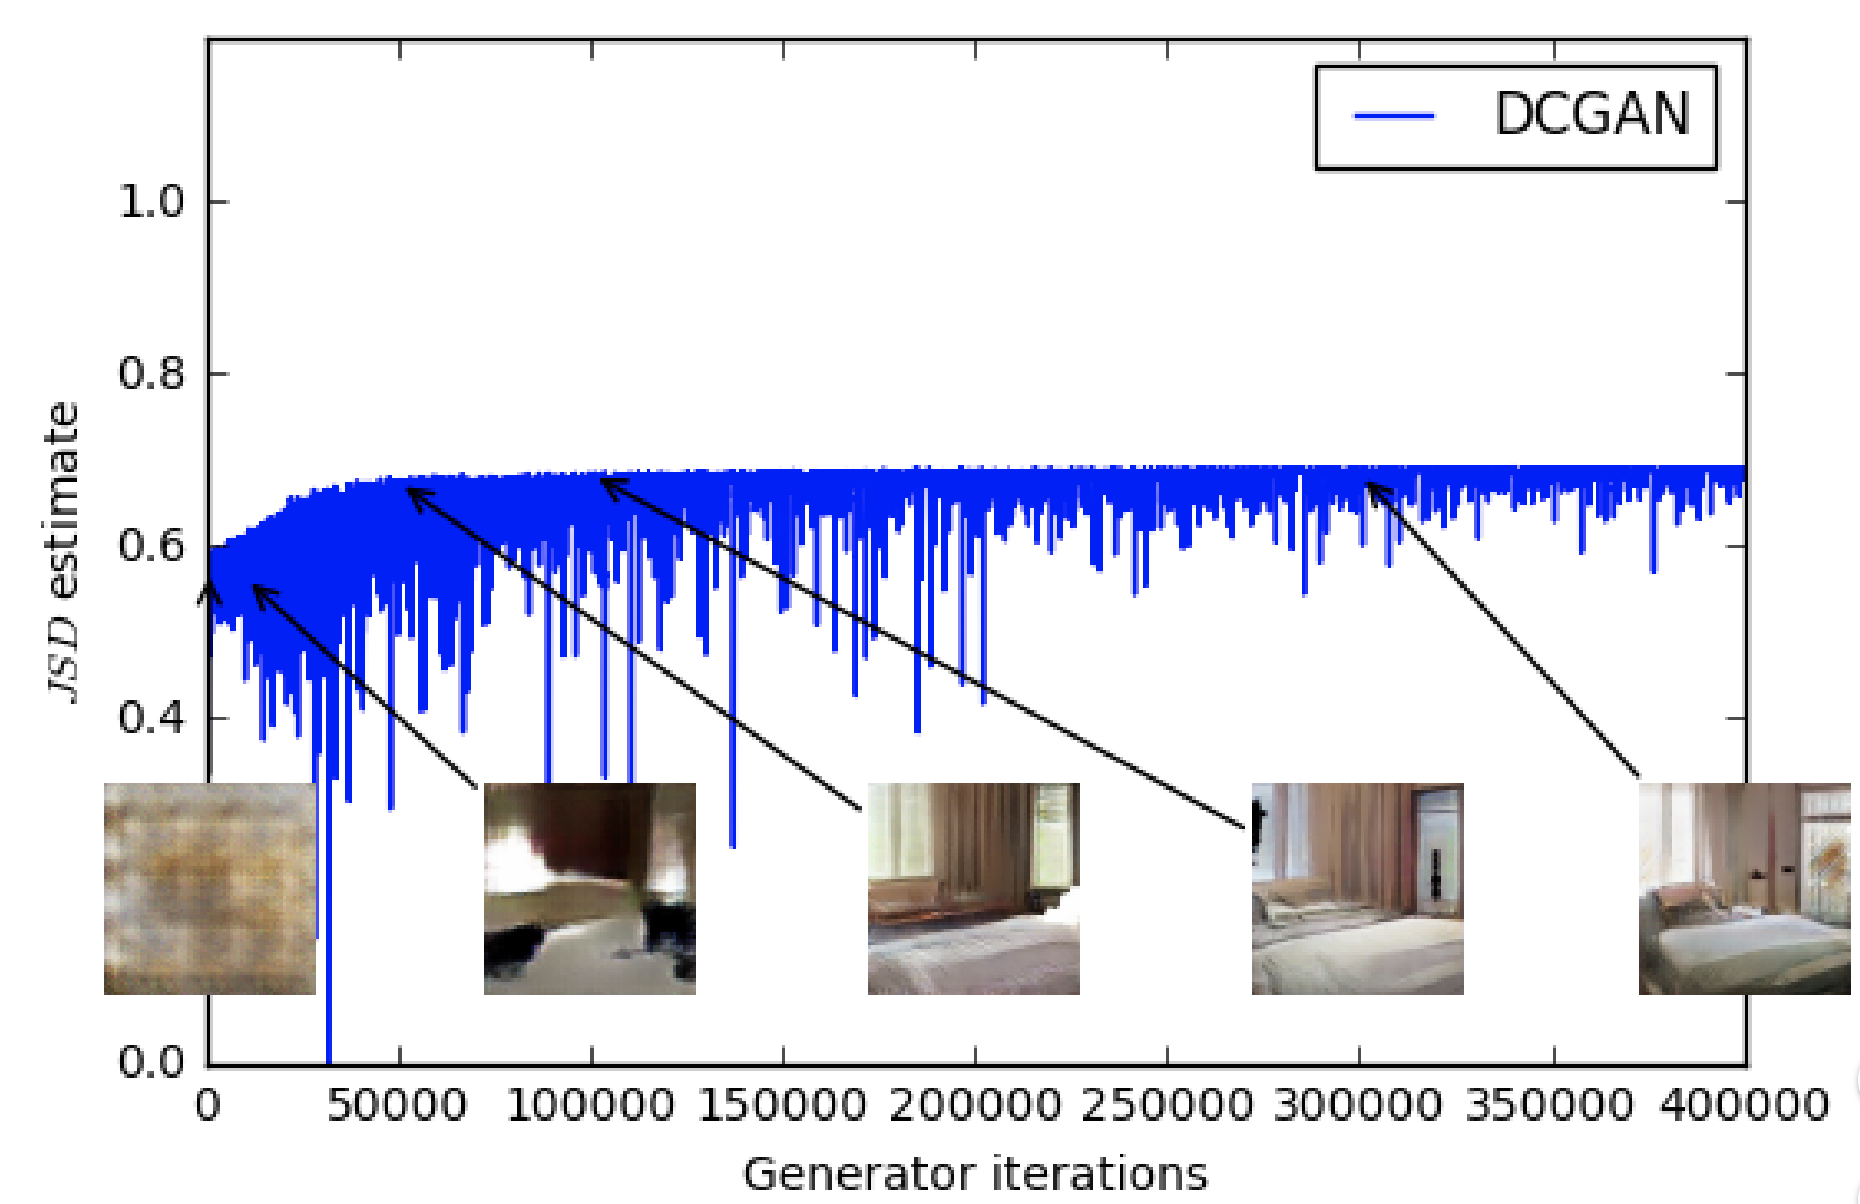
\includegraphics[width=1.0\linewidth]{figs/dcgan_quality}
		\end{figure}
	\end{minipage}%
	\begin{minipage}[t]{0.5\columnwidth}
		\begin{figure}
			\centering
			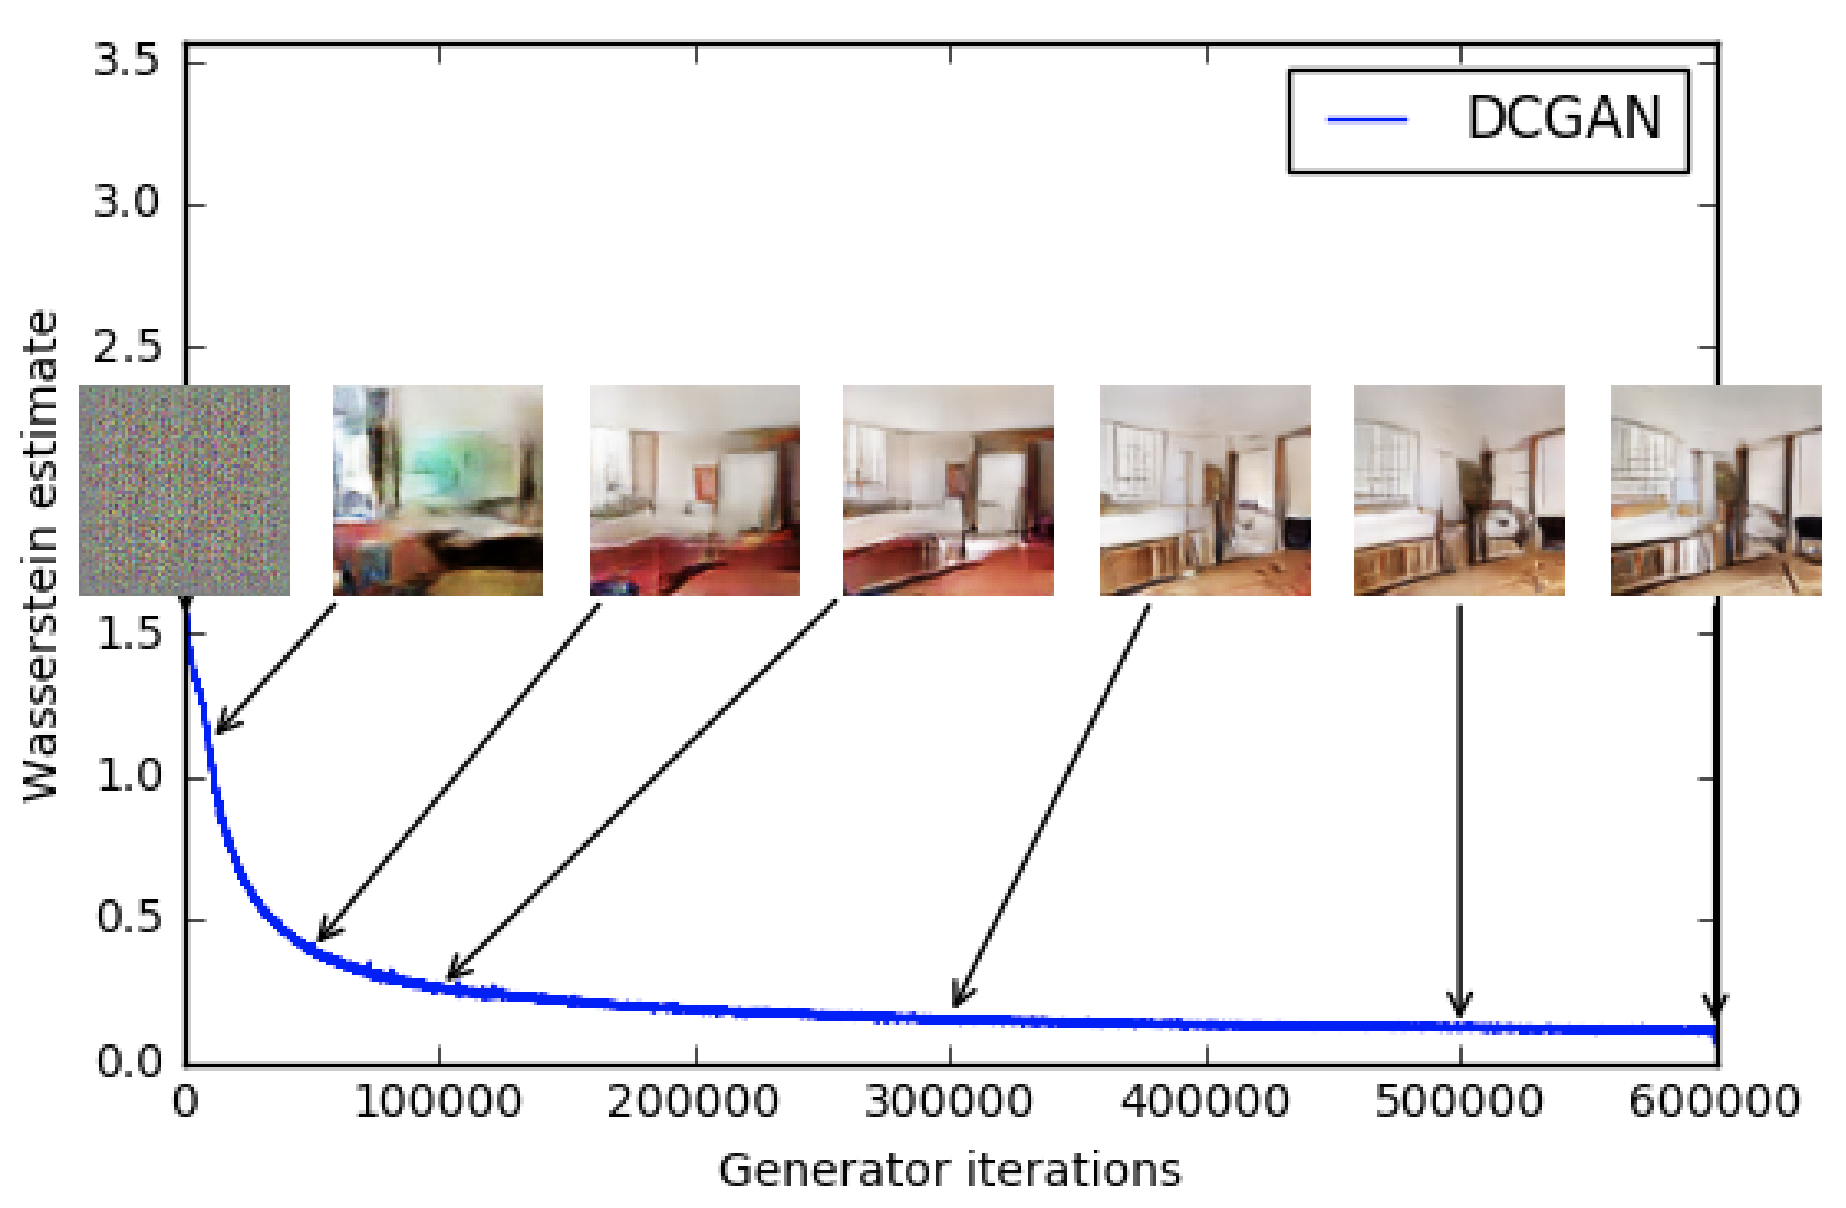
\includegraphics[width=1.0\linewidth]{figs/wgan_quality}
		\end{figure}
	\end{minipage}
	
	\myfootnotewithlink{https://arxiv.org/abs/1701.07875}{Arjovsky M., Chintala S., Bottou L. Wasserstein GAN, 2017}
\end{frame}
%=======
\subsection{WGAN with Gradient Penalty}
%=======
\begin{frame}{Wasserstein GAN with Gradient Penalty}
	\vspace{-0.2cm}
	\begin{figure}
		\centering
		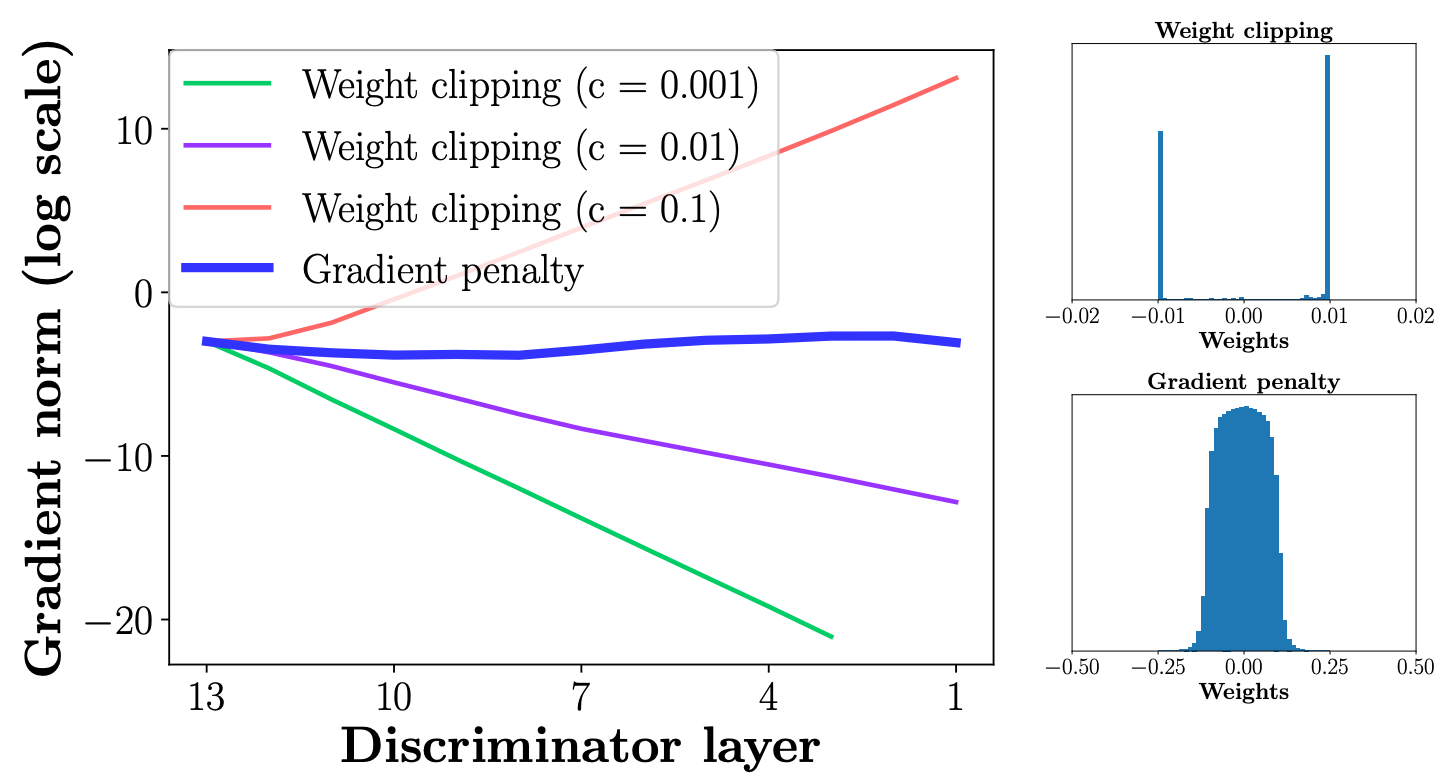
\includegraphics[width=0.9\linewidth]{figs/wgan_gp_weights}
	\end{figure}
	\vspace{-0.2cm} 
	
	\begin{block}{Weight clipping analysis}
		\begin{itemize}
			\item The gradients either grow or decay exponentially.
			\item Gradient penalty makes the gradients more stable.
		\end{itemize}
	\end{block}
	\myfootnotewithlink{https://arxiv.org/abs/1704.00028}{Gulrajani I. et al. Improved Training of Wasserstein GANs, 2017}
\end{frame}
%=======
\begin{frame}{Wasserstein GAN with Gradient Penalty}
	\begin{block}{Theorem}
		Let $\pi(\bx)$ and $p(\bx)$ be two distribution in $\cX$, a compact metric space. Let $\gamma$ be the optimal transportation plan between $\pi(\bx)$ and $p(\bx)$. Then
		\begin{enumerate}
			\item there is 1-Lipschitz function $f^*$ which is the optimal solution of 
			\[
				\max_{\| f \|_L \leq 1} \left[ \bbE_{\pi(\bx)} f(\bx)  - \bbE_{p(\bx)} f(\bx)\right].
			\]
			\item if $f^*$ is differentiable, $\gamma(\by = \bz) = 0$ and $\hat{\bx}_t = t \by + (1 - t) \bz$ with $\by \sim \pi(\bx)$, $\bz \sim p(\bx | \btheta)$, $t \in [0, 1]$ it holds that
			\[
				\bbP_{(\by, \bz) \sim \gamma} \left[ \nabla f^*(\hat{\bx}_t) = \frac{\bz - \hat{\bx}_t}{\| \bz - \hat{\bx}_t \|} \right] = 1.
			\]
		\end{enumerate}
	\end{block}
	\vspace{-0.5cm}
	\begin{block}{Corollary}
		$f^*$ has gradient norm 1 almost everywhere under $\pi(\bx)$ and $p(\bx)$.
	\end{block}

	\myfootnotewithlink{https://arxiv.org/abs/1704.00028}{Gulrajani I. et al. Improved Training of Wasserstein GANs, 2017}
\end{frame}
%=======
\begin{frame}{Wasserstein GAN with Gradient Penalty}
	A differentiable function is 1-Lipschtiz if and only if it has gradients with norm at most 1 everywhere.
	\begin{block}{Gradient penalty}
		\vspace{-0.3cm}
		\[
			W(\pi || p) = \underbrace{\bbE_{\pi(\bx)} f(\bx)  - \bbE_{p(\bx)} f(\bx)}_{\text{original critic loss}} + \lambda \underbrace{\bbE_{U[0, 1]} \left[ \left( \| \nabla f(\hat{\bx}) \|_2 - 1 \right) ^ 2\right]}_{\text{gradient penalty}},
		\]
		\vspace{-0.3cm}
	\end{block}
	\begin{itemize}
		\item Samples $\hat{\bx}_t = t \by + (1 - t) \bz$ with $t \in [0, 1]$ are uniformly sampled along straight lines between pairs of points: $\by$ from the data distribution $\pi(\bx)$ and $\bz$ from the generator distribution $p(\bx | \btheta)$.
		\item Enforcing the unit gradient norm constraint everywhere is intractable, it turns out to be sifficient to enforce it only along these straight lines.
	\end{itemize}

	\myfootnotewithlink{https://arxiv.org/abs/1704.00028}{Gulrajani I. et al. Improved Training of Wasserstein GANs, 2017}
\end{frame}
%=======
\begin{frame}{Summary}
	\begin{itemize}
		\item GAN tries to optimize Jensen-Shannon divergence (in theory).
		\vfill
		\item Mode collapse is one of the main problems of vanilla GAN.  Lots of tips and tricks has to be used to make the GAN training is stable and scalable.
		\vfill
		\item KL and JS divergences work poorly as model objective in the case of disjoint supports.
		\vfill
		\item Earth-Mover distance is a more appropriate objective function for distribution matching problem.	
		\vfill
		\item Kantorovich-Rubinstein duality gives the way to calculate the EM distance using only samples.
		\vfill
		\item Wasserstein GAN uses Kantorovich-Rubinstein duality for getting Earth Mover distance as model objective.
		\vfill
		\item Weight clipping is a terrible way to enforce Lipschitzness. Gradient Penalty adds regularizer to loss that uses neccessary conditions for optimal critic.
	\end{itemize}
\end{frame}
\end{document} 